\PassOptionsToPackage{hyphens}{url}
\documentclass{article}
\usepackage[preprint]{neurips_2026}

\usepackage[T1]{fontenc}
\usepackage[utf8]{inputenc}
\usepackage{textcomp}
\usepackage{amsmath,amssymb}
\usepackage{booktabs,array,longtable}
\usepackage{calc}
\usepackage{graphicx}
\usepackage{xcolor}
\usepackage{xurl}
\usepackage{microtype}
\usepackage{hyperref}
\usepackage{bookmark}

\graphicspath{{figures/}}
\setcounter{secnumdepth}{3}
\setcounter{tocdepth}{2}
\setlength{\emergencystretch}{3em}
\providecommand{\tightlist}{\setlength{\itemsep}{0pt}\setlength{\parskip}{0pt}}

\hypersetup{
  pdftitle={Neural Network Training as Key Search Across Resolution Bands},
  pdfauthor={Jurij Jukic},
  hidelinks,
  pdfcreator={LaTeX}
}

\title{Neural Network Training as Key Search Across Resolution Bands}
\author{%
  Jurij Juki\'c\\
  Independent Researcher\\
  Zagreb, Croatia\\
  \texttt{j.jjukicc@gmail.com}
}
\date{}

\begin{document}
\maketitle

\begin{abstract}
Scalar loss in machine learning obscures what a neural network learns
and when. While the specific circuits in a network are opaque, we can
observe how a network learns across different resolutions of data.
Our hope is that our resolution-based approach makes theories of
learning easier to formulate and test. We illustrate this by proposing
a phenomenological model, key search, with a concrete methodology that decomposes
the learning process across three axes: parameter time, resolution band,
and band loss. Parameter time is a reparameterization of training time
by distance traveled along the optimizer's path in parameter space. A
resolution band is the content present at a higher resolution level but
absent at a lower one, obtained as an orthogonal component of a
multiresolution analysis. Band loss is the loss restricted to that band,
rather than the full resolution. Key search predicts three results,
which we test on 12 CelebA $64\times 64$ autoencoding runs (6 CNN, 6 ViT): 1.
the gap between a band's current loss and its floor is well fit by a
Weibull curve in parameter time over the active window ($R^2 >
0.99$ for bands 2--64); 2. band activation is ordered across scales, with
finer bands activating later (Spearman $\rho = 0.79$), decaying over wider
parameter time windows ($\rho = 0.96$), reaching higher floors ($\rho = 0.96$),
and starting with smaller removable loss ($\rho = -0.89$); 3. the ordinary
scalar loss, obtained by summing band residuals, is also well
summarized by a single Weibull curve in parameter time (median
$R^2 = 0.996$, median $\Delta\mathrm{BIC} = -28.83$ versus exponential).

\end{abstract}

\section{Introduction}\label{intro}

A neural network's training loss is a single scalar that hides
everything about what the network is learning and when. This paper asks
whether decomposing that scalar into interpretable components can reveal
structure in the learning process that the aggregate curve obscures.

We study image autoencoders, where a natural decomposition is available:
the Haar wavelet basis splits an image into orthogonal resolution bands,
each capturing the content present at one spatial scale but absent at the
next coarser one. Because the bands are orthogonal and the loss is
squared error, band losses sum exactly to total loss. This lets us track
how much of the learning at any point in training is happening at each
resolution, rather than observing only the aggregate.

Alongside this decomposition, we introduce a second methodological
choice: measuring training progress not in raw step count but in
parameter time --- the cumulative Euclidean distance traveled by the
parameters. The intuition is that parameter distance tracks how far the
optimizer has actually searched, whereas raw step count confounds search
progress with the optimizer's varying step size.

With these two tools --- band decomposition and parameter time --- we
propose and test a phenomenological model we call key search. The idea
is that training searches for keys: parameter
configurations that unlock loss reduction at a given resolution band.
Short keys are easy to find and tend to be effective (coarse structure
accounts for large chunks of loss); long keys take more search and yield
smaller returns (fine detail is particular and accounts for less loss).
From this picture, three predictions follow:

\begin{enumerate}
\item \textbf{Shape.} Each band's residual --- the difference between current
  loss and final loss --- follows a Weibull decay in parameter
  time, reflecting a search process whose rate changes over time.
\item \textbf{Ordering.} Coarse bands activate earlier, achieve their final loss sooner,
  reach lower floors, and have more total removable loss than fine bands.
\item \textbf{Full-loss residual.} The full-loss scalar residual, which
  is the sum of the band residuals, is also well described by a single
  Weibull curve in parameter time.
\end{enumerate}

We test these predictions on 12 CelebA $64\times 64$ autoencoding runs
(6~CNN, 6~ViT). All three are supported in this setting: per-band Weibull fits achieve
$R^2 > 0.99$ for bands 2--64; ordering across bands holds with Spearman
$\rho$ between 0.79 and 0.96 on all four measured quantities; and the
full-loss Weibull fit achieves median $R^2 = 0.996$ with
$\Delta\mathrm{BIC} = -28.83$ versus the exponential special case.

Our hope is that the methodology --- band decomposition plus parameter
time --- is useful independently of the specific theory tested here.
Decomposing loss into orthogonal components, each with
its own trajectory, provides a richer set of observables against which
theories can be checked.

\section{Related work}\label{related-work}

\paragraph{Scaling laws.}
\citet{kaplan2020scaling} established that language model loss follows power
laws in model size, dataset size, and compute; \citet{hoffmann2022training}
revised the compute-optimal tradeoff. Subsequent work has sought
theoretical explanations for these power-law exponents
\citep{bahri2024explaining,sharma2022scaling}. These analyses fit a single scalar loss
against raw training step or compute. Our work differs in two respects:
we decompose loss by resolution band before fitting, and we
reparameterize training time as cumulative parameter-space distance
rather than step count. The resulting per-band curves are Weibull rather
than power law.

\paragraph{Spectral bias and the frequency principle.}
\citet{rahaman2019spectral} and \citet{xu2020frequency} independently showed
that neural networks learn low-frequency components of the target
function before high-frequency ones, a phenomenon called spectral bias
or the frequency principle (F-Principle). Our band-ordering result
(Result~2) is a counterpart of this observation on images analyzed with Haar wavelets: coarse
bands are learned before fine bands. However, our focus is different.
The spectral bias literature characterizes \emph{which} frequencies are
learned first; we additionally measure \emph{how much loss} each band
contributes, fit a parametric decay curve to the per-band dynamics, and
connect the ordering to a theoretical framework (key search).

\paragraph{Bennett's logical depth.}
\citet{bennett1988logical} defined the logical depth of an object in
terms of the time required by a near-shortest program to produce it,
formalizing the distinction between
objects that are merely information-rich and those that are
computationally expensive to produce. \citet{hoang2018deep}
conjectured that deep learning succeeds because real-world data has
large non-parallelizable logical depth, connecting Bennett's notion to
network depth (number of layers). Our use of logical depth is different:
we use it to motivate a model of training \emph{dynamics}, where depth
corresponds to the parameter-time of finding a loss-reducing key,
not to architectural depth.

\paragraph{Parameter-space geometry.}
The geometry of training trajectories has been studied through loss
landscape visualization \citep{li2018visualizing} and the low-dimensional
structure of gradient updates \citep{gurari2018gradient}. Our parameter
time $s(t)$ --- cumulative Euclidean distance in parameter space --- is
related in spirit to these geometric views, but we use it as a
reparameterized training time under which per-band losses become clean
Weibull curves. To our knowledge, cumulative parameter distance has not
previously been used as a time axis for fitting training dynamics.

\paragraph{Learning curve functional forms.}
In the machine learning scaling law literature, power laws are the dominant
functional form \citep{kaplan2020scaling,hoffmann2022training}. We are
not aware of prior work fitting Weibull curves to neural network
training loss, though the Weibull distribution appears in survival
analysis and reliability engineering.

\section{Setup}\label{setup}

\paragraph{Resolution.} We use \emph{resolution} to refer to spatial scale in a
multiresolution decomposition. A resolution level $r$ corresponds to an
$r\times r$ spatial grid. We work with dyadic levels
$r\in\{1,2,4,8,16,32,64\}$ for our CelebA $64\times 64$ images.

\paragraph{Resolution band.} For an image at resolution $N\times N$, a resolution band
captures the content added at a specific spatial scale. Concretely, we
use the Haar decomposition to split an image into nested resolutions:
the coarsest level captures global block averages, each finer level
captures the detail added relative to the coarser one. For a $64\times 64$
image, this yields 7 bands at dyadic resolutions (1, 2, 4, 8, 16, 32,
64), each orthogonal to the others.

\paragraph{Band loss.} The loss a model achieves at a given resolution band. In
general, band losses need not sum to total loss; whether they do depends
on the loss function and the decomposition. When the bands are
orthogonal (the content at each finer band is orthogonal to all content
at coarser ones) and the loss is squared-error, the band losses sum
exactly to the total loss. For an input image $x$ and model reconstruction
$f(x;\theta_t)$ at training time $t$,

\begin{equation}\label{eq:additivity}
\mathrm{MSE}(x, f(x;\theta_t)) = \sum_i L_i(x, f(x;\theta_t)).
\end{equation}

For this reason, we restrict our empirical study to image reconstruction
with MSE loss. Formal definitions and derivation are given in Appendix~\ref{app:haar-decomposition}.

\paragraph{Floor.} For each band $i$, we denote its floor, the final achieved loss as $L_i^\infty$ 
(estimated from saturated late-training behavior).

\paragraph{Residual.} We then define residual-to-floor as

\begin{equation}\label{eq:residual}
R_i(t) = L_i(t) - L_i^\infty,
\end{equation}

This is the amount of removable loss still remaining in band $i$ at time
t, decaying to zero as training saturates.

Because the Haar bands are orthogonal and the loss is MSE, the
ordinary full-resolution loss is the sum of the band losses. We therefore
define the full-loss residual, also called the total residual, as
\[
R_{\mathrm{tot}}(t)
=
\sum_i R_i(t)
=
\sum_i \left(L_i(t)-L_i^\infty\right).
\]

Equivalently,
\[
R_{\mathrm{tot}}(t) = L_{\mathrm{tot}}(t) - L_{\mathrm{tot}}^\infty,
\]
where $L_{\mathrm{tot}}^\infty = \sum_i L_i^\infty$.

\paragraph{Raw time.} We use $t$ to denote the training step count.

\paragraph{Parameter time.} Parameter-space distance measures how much the model's
parameters have moved. We define parameter time $s(t)$ as the
cumulative parameter-space distance along the optimizer's trajectory up
to raw training step $t$:

\[
s(t) = \sum_{k=1}^{t} \| \theta_k - \theta_{k-1} \|,
\]

where $\theta_k$ denotes the model's parameters at step $k$.

Empirically, the relationship between parameter time and raw time $t$ is
approximately power-like:
\[
s(t) \approx a + b t^\gamma,
\]
with median $\gamma = 0.368$, run-to-run SD $= 0.008$, and median
full-window $R^2 = 0.999$. More in Appendix~\ref{app:optimizer-path-measurements}.

\begin{figure}
\centering
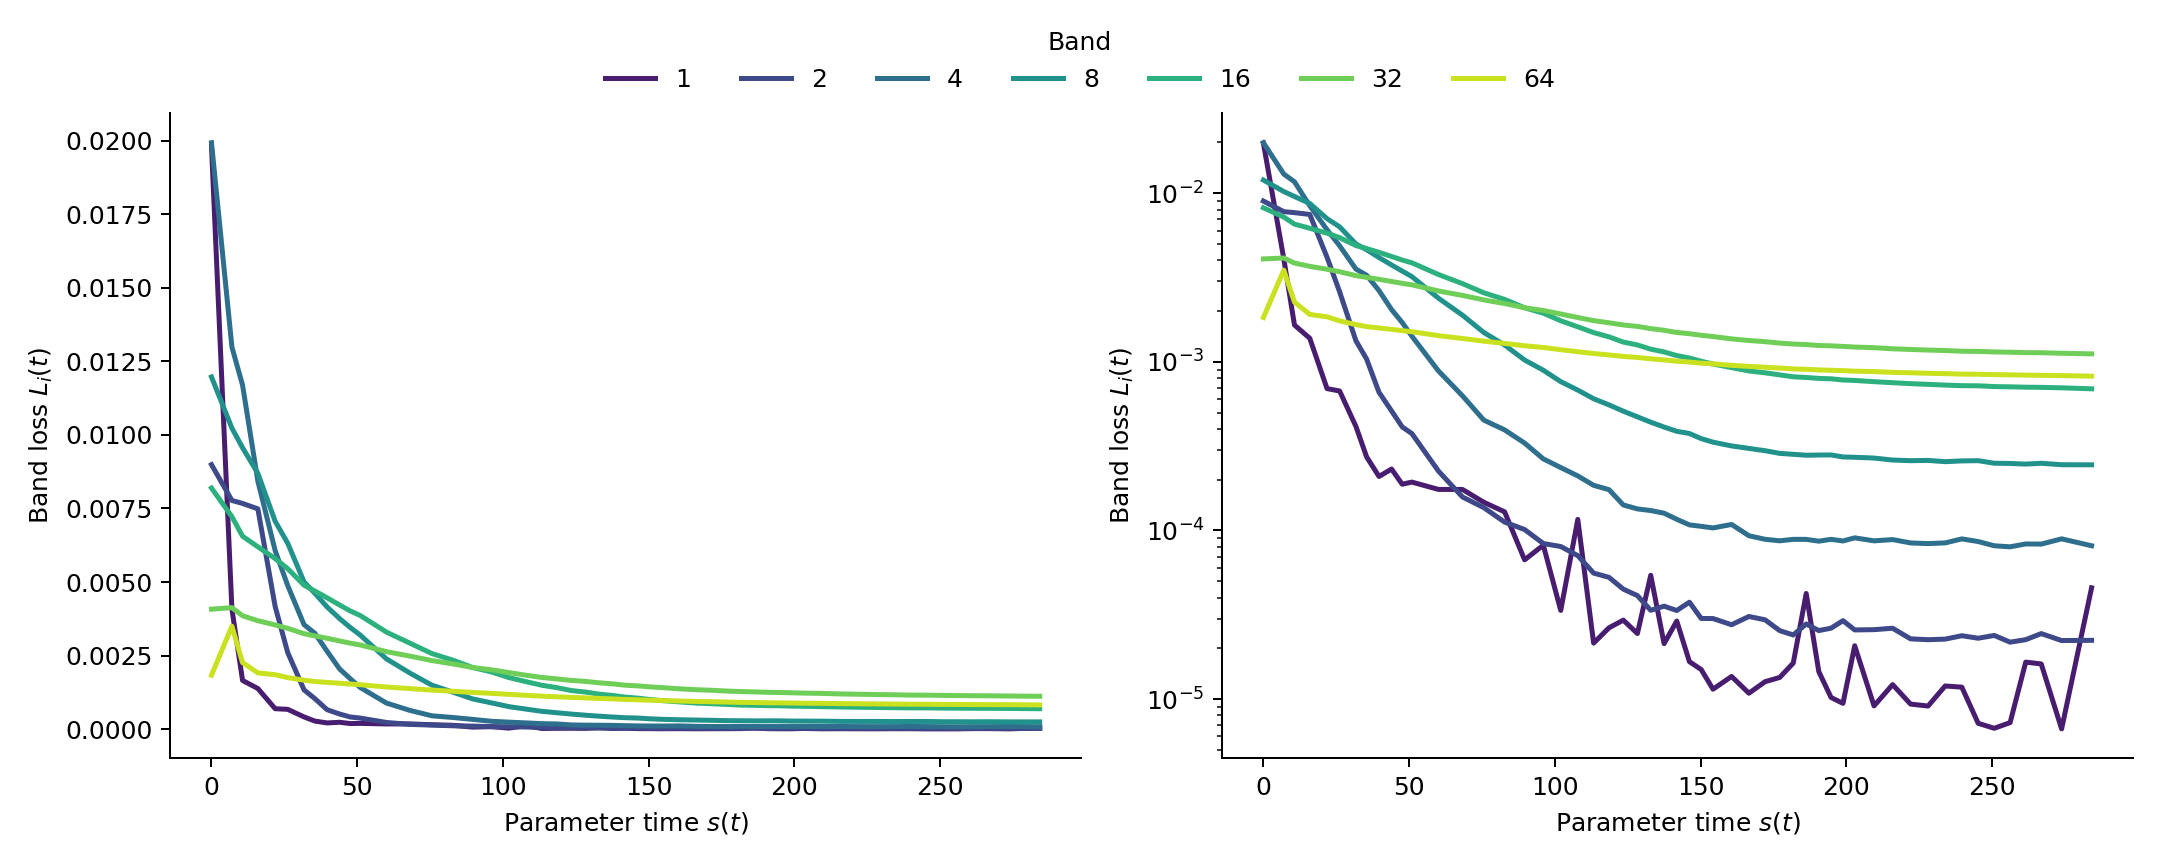
\includegraphics[width=\linewidth]{figure1.png}
\caption{Band loss $L_i$ over parameter time $s$ for one
CelebA ViT autoencoding run, with each line corresponding to one
resolution band. Left: linear y-axis. Right: log y-axis.}
\label{fig:band-loss}
\end{figure}

\section{Theory}\label{theory}

\subsection{Key search}\label{key-search}

This section motivates the theoretical constructs we use and
informally introduces the main quantities we measure.

Bennett's logical depth formalizes the intuition that some structures
are not merely information-rich but computationally expensive to
produce. He compares two quantities: a string's Kolmogorov
complexity is the length of the shortest program that generates it, and
its depth is the runtime of that program. A random string has high
K complexity (no short program exists) but low depth (it is copied
verbatim). The digits of $\pi$ have low K complexity (a short formula
generates them) but high depth (the formula takes long to run).

Bennett's insight connects depth to search cost: short programs of
length $\ell$ are rare among the $2^\ell$ candidates of that length,
and so take long to find by enumeration. A deep string is one that cannot
be produced without finding such rare, hard-to-find programs.

We adopt this framing for neural network training and postulate that
training searches for keys: programs that reduce loss at a given
resolution band. For each key, we distinguish its depth (the parameter
time required to find it) from its effectiveness (the loss reduction
once found). From this idea, three predictions follow.

\paragraph{Prediction 1 (shape).} The search process itself has a characteristic
shape. In a simple search for a key of length $\ell$, the per-step
probability of finding it is roughly $2^{-\ell}$. Assuming independent
trials, the probability that the key has not yet been found after $t$
steps is $(1 - 2^{-\ell})^t$, which decays exponentially in
$t$. We relate this remaining probability to the residual loss $R_i(t)$.
However, real training is not a simple search. Keys roughly correspond
to parameter configurations, and gradient descent follows the loss
landscape: keys in steep, easily-descended regions are reached first;
those in flatter or more distant regions take longer. Therefore, the 
rate at which keys are found need not remain constant
over time, and the residual need not decay at a constant rate. The
resulting residual is not expected to be a pure exponential. We model
it with the Weibull family, a generalization of the exponential that
allows the decay rate to speed up or slow down over time.

These ideas also motivate our choice of parameter time. Parameter time
reflects how far the search has actually traveled in parameter space, i.e.
different keys or parameter configurations that have been tried,
which we presume tracks search progress more accurately than raw
training step count.

\paragraph{Prediction 2 (ordering).} Across bands, depth and effectiveness tend to
inversely correlate. Shallow keys tend to be more effective. For example, at
$2\times 2$ or $4\times 4$, a short program capturing overall face structure reduces the
band's loss by a large amount. Deep keys tend to be less effective,
since fine-scale structure is more particular and accounts for a smaller
chunk of total loss. This gives a pattern across bands: coarse bands
begin learning early (shortest effective key is shorter than for fine bands)
and reduce loss by a large margin (more removable loss than fine bands).

\paragraph{Prediction 3 (full-loss residual).} The same
key-search logic that applies to each band applies to the full loss: the
aggregate training process is also a search over keys, so the full-loss
residual should also follow a Weibull decay in parameter time. 
Moreover, because the band losses are additive, the ordinary scalar
residual is the sum of the band residuals. The Weibull family is not closed
under summation, so a sum of per-band Weibulls need not itself be
Weibull-shaped. Nevertheless, we find that a single Weibull fits the
full-loss residual well (Result 3). 

\begin{figure}[h!]
\centering
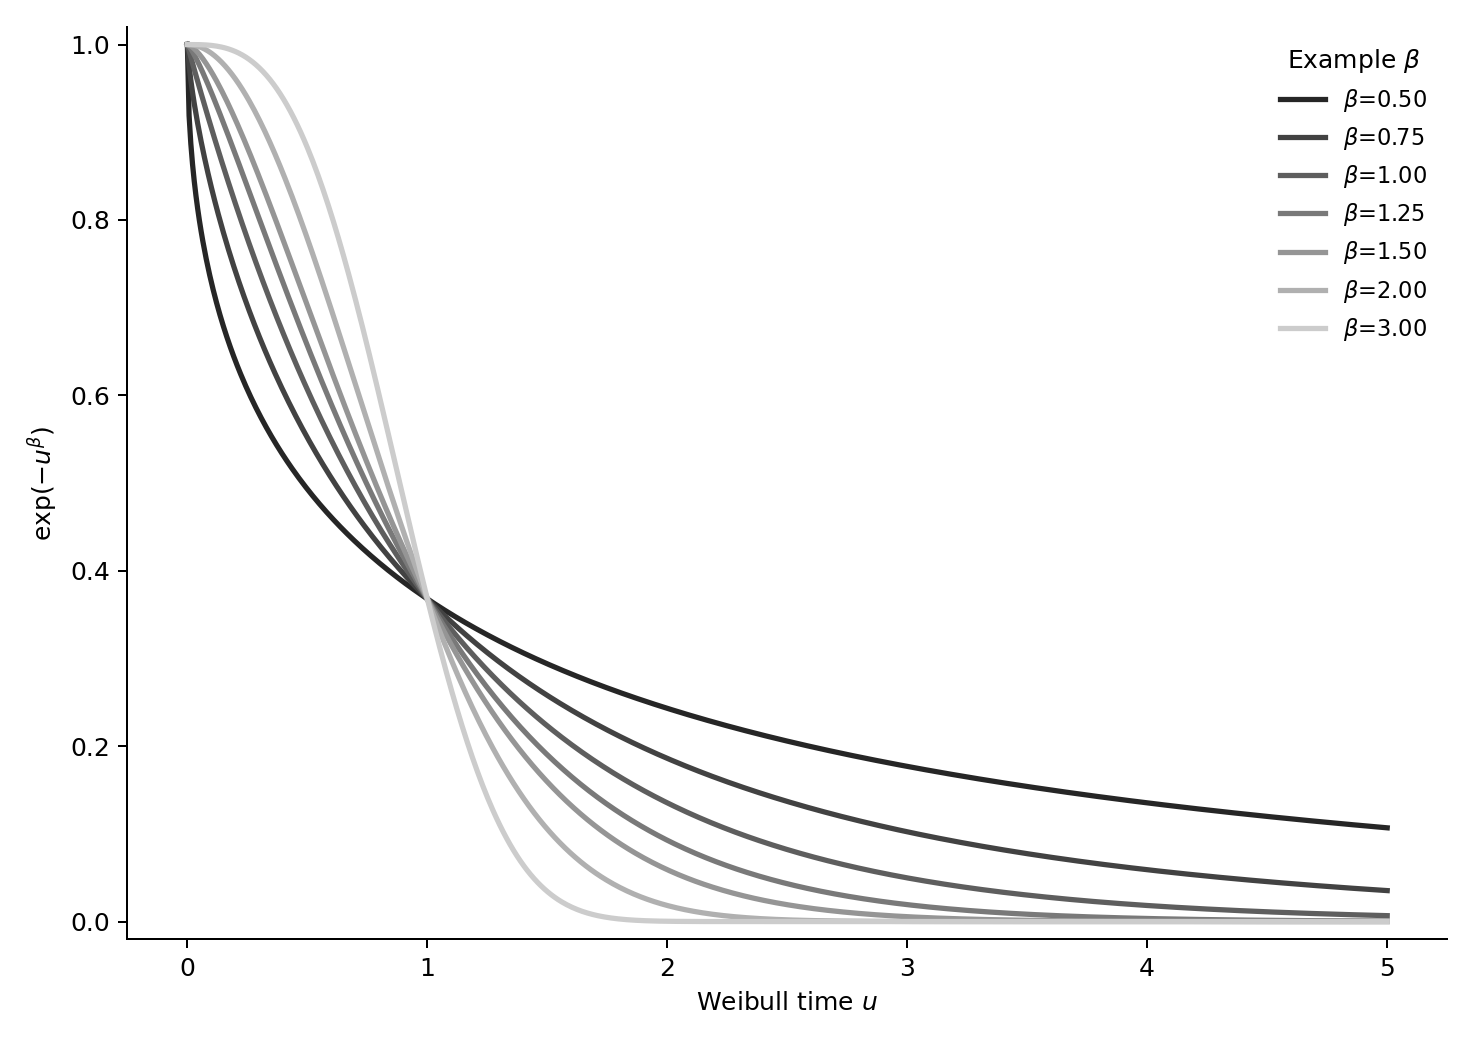
\includegraphics[width=0.6\linewidth]{figure2.png}
\caption{To illustrate how the Weibull $\beta$ parameter shapes the decay curve, this figure shows
stylized Weibull curves for different $\beta$ values (schematic, not a fit to
data). For $\beta = 1$, the curve is a pure exponential. For $\beta < 1$,
decay is fast initially then slows (diminishing returns). For $\beta > 1$,
decay is initially slow --- a ``warmup'' phase ---
followed by faster decay.}
\label{fig:weibull-shapes}
\end{figure}

\subsection{Residual as a Weibull tail}\label{residual-as-a-weibull-tail}

We refer to Prediction 1 from the key search section, where we postulate
that the residual follows a Weibull-shaped tail. We define the
band's tail $T_i$ as

\begin{equation}\label{eq:weibull-tail}
T_i(x)=A_i^{\mathrm{tail}}\exp\!\left(-(x/\omega_i)^{\beta_i}\right)
\quad\text{for } x \ge 0,
\end{equation}

where $A_i^{\mathrm{tail}}$ is the theoretical tail amplitude, $\omega_i$ is a
scale parameter, and $\beta_i$ is the Weibull shape exponent. The
argument $x$ is not training time itself, it represents search progress or
frontier position along the tail.

Let $x_i(t)$ denote the frontier position for band $i$. Then the band's
residual is

\[
R_i(t) = T_i(x_i(t)).
\]

The frontier $x_i$ depends on the band's data, the learner, and training
time --- different learners applied to the same data would progress
along the tail at different rates. This separates the tail (a property
of the data) from the frontier (how the specific learner moves along
it).

The frontier $x_i$ is latent and not directly measured. We therefore
cannot directly observe the Weibull shape in $x$-space. What we can
observe is $R_i$ as a function of parameter time $s$.

The separation between tail and frontier is a conceptual clarification,
not an empirical decomposition. The frontier $x_i$ is latent and not
directly measured; in this paper we fit Weibull curves directly to $R_i(s)$
and do not attempt to recover $x_i$. If the frontier is a monotonic power-like
function of $s$, then a Weibull in $x$ manifests as a Weibull in $s$. 
We find that it does: the fitted Weibull describes
band residuals well (Result~1). Whether
parameter time is a good proxy for frontier position across
architectures and datasets remains an open question; we observe only
that it produces clean fits for our CNN and ViT runs on CelebA.

\section{Experimental Setup and Measurement Protocol}
\label{experimental-setup}

We study training dynamics in image autoencoding on CelebA ($64\times 64$). We
train 12 runs total: 6 CNN and 6 ViT, using seeds 45--50 for each
architecture. The CNN is a 4-layer strided convolutional autoencoder
(1.83M parameters); the ViT uses 4 transformer layers with $4\times 4$ patches
(2.78M parameters). Both use a 128-dimensional latent and Sigmoid
output. Training uses plain Adam (lr=$3\times10^{-4}$, batch size 128) for 50
epochs, with no learning-rate schedule, no weight decay, and no gradient
clipping. Band losses $L_i(s)$ are computed on a fixed 256-image
test panel per run.

Parameter time $s(t)$ is the cumulative sum of Euclidean distances
between successive saved checkpoints. The residual is
$R_i(s)=L_i(s)-L_i^\infty$, where the floor $L_i^\infty$ is estimated as
the mean band loss over the last five saved checkpoints.
Appendix~\ref{app:floors} checks that replacing the average by the final
checkpoint gives nearly identical floors.

\subsection{Threshold crossings}\label{threshold-crossings}
Our measurements are available only at a finite set of saved checkpoints,
indexed by $k$, with parameter times $s_k$. For band $i$, define
the normalized residual at checkpoint $k$ as

\[
q_i(s_k)=\frac{R_i(s_k)}{R_i(s_0)},
\]
where $s_0$ denotes the initial checkpoint.

For threshold $\alpha\in(0,1)$, the \(\alpha\)-crossing
$c_i(\alpha)$ is the parameter-time location at which $q_i$ first
falls below \(\alpha\), estimated by linear interpolation between the two
adjacent saved checkpoints that bracket the threshold. The interpolation
formula is given in Appendix~\ref{app:crossings}. Crossings are used for two purposes. 

\paragraph{Band ordering.} Crossings define the quantities that describe
band-ordering: onset is the 0.95 crossing, i.e. the parameter time at which the
band has achieved the first 5\% of its loss reduction:

\[
\tau_i=c_i(0.95),
\]

and active width is the distance between the 0.95 and 0.01 crossings, the length
of time during which the band has achieved most of its loss reduction:

\[
w_i=c_i(0.01)-c_i(0.95).
\]

\paragraph{Active windows for Weibull fits.}
For each per-band fit, the active window begins at the first saved
checkpoint after $c_i(0.95)$ and ends at the last saved checkpoint
before $c_i(0.01)$. This threshold pair is fixed before fitting rather
than chosen to optimize fit quality. Thus the crossings define the window
boundaries, but the fitted data are only the saved checkpoint observations
inside that window. Direct global fits are single Weibull fits to the
full-loss residual $R_{\mathrm{tot}}$. Full-loss fits do not use crossing-defined
active windows; they use the full saved-checkpoint range.

\subsection{Fit quality}\label{fit-diagnostics-and-model-comparison}

Reported $R^2$ values are computed directly on the residual values $R_i(s)$ in the
same linear scale used by MSE, not on the log scale.

For model comparison we report
\[
\Delta\mathrm{BIC}
=
\mathrm{BIC}_{\mathrm{Weibull}}
-
\mathrm{BIC}_{\mathrm{exp}},
\]
which penalizes the Weibull's extra shape parameter $\beta$ unless it
earns its keep through better fit. Negative values favor Weibull over
the exponential special case ($\beta=1$).

Full architecture specifications, checkpoint schedule, crossing
interpolation formula, fit procedure, and robustness analyses are given
in Appendices~\ref{appendix:experimental-details} and~\ref{appendix:weibull-fit-details}.

\section{Results}\label{results}

\subsection{Result 1: Weibull}\label{result-1-weibull}

Figure~\ref{fig:band-loss} shows that band trajectories do not necessarily decay smoothly
from the start of training. Band 64 rises above its initial value before
decaying; band 32 shows a small early bump; coarse bands such as band 2
drop almost immediately. In the key-search framing, this corresponds to
a pre-decay phase before the optimizer has reached a key that produces
useful loss reduction in that band.

For this reason, we do not fit Weibulls to the full per-band trajectory.
Instead, for each band we fit only the checkpoint observations inside
the active window defined in Section~\ref{experimental-setup}: the first
saved checkpoint after the 0.95 crossing through the last saved
checkpoint before the 0.01 crossing. No interpolated residual values are
used in the fit.

We fit the Weibull tail form of Eq.~\eqref{eq:weibull-tail} to each band's residual
trajectory $R_i(s)$ using nonlinear least squares with
bounds on each parameter.

We obtain $R^2 > 0.99$ across bands 2--64, with band 1 at $R^2 = 0.982$ (Appendix~\ref{app:per-band-weibull-vs-exponential}). To assess whether the additional Weibull shape parameter
is warranted, we compare Weibull fits against the pure exponential special case
$\beta = 1$ via BIC. Weibull is preferred with median $\Delta\mathrm{BIC} = -19.65$ (72/84 fits);
under a conservative $n_{\mathrm{eff}} = n/10$ deflation accounting for hidden
correlations, Weibull preference still holds at median
$\Delta\mathrm{BIC} = -1.73$ (78/84 fits). Fits are performed in parameter
time. The active-window choice is not critical: under alternative
0.90/0.10 and 0.80/0.20 threshold windows, fit quality remains stable
and the band ordering correlations (shown in the following section) are essentially unchanged
(Appendix~\ref{app:fit-window-robustness}).

\begin{figure}
\centering
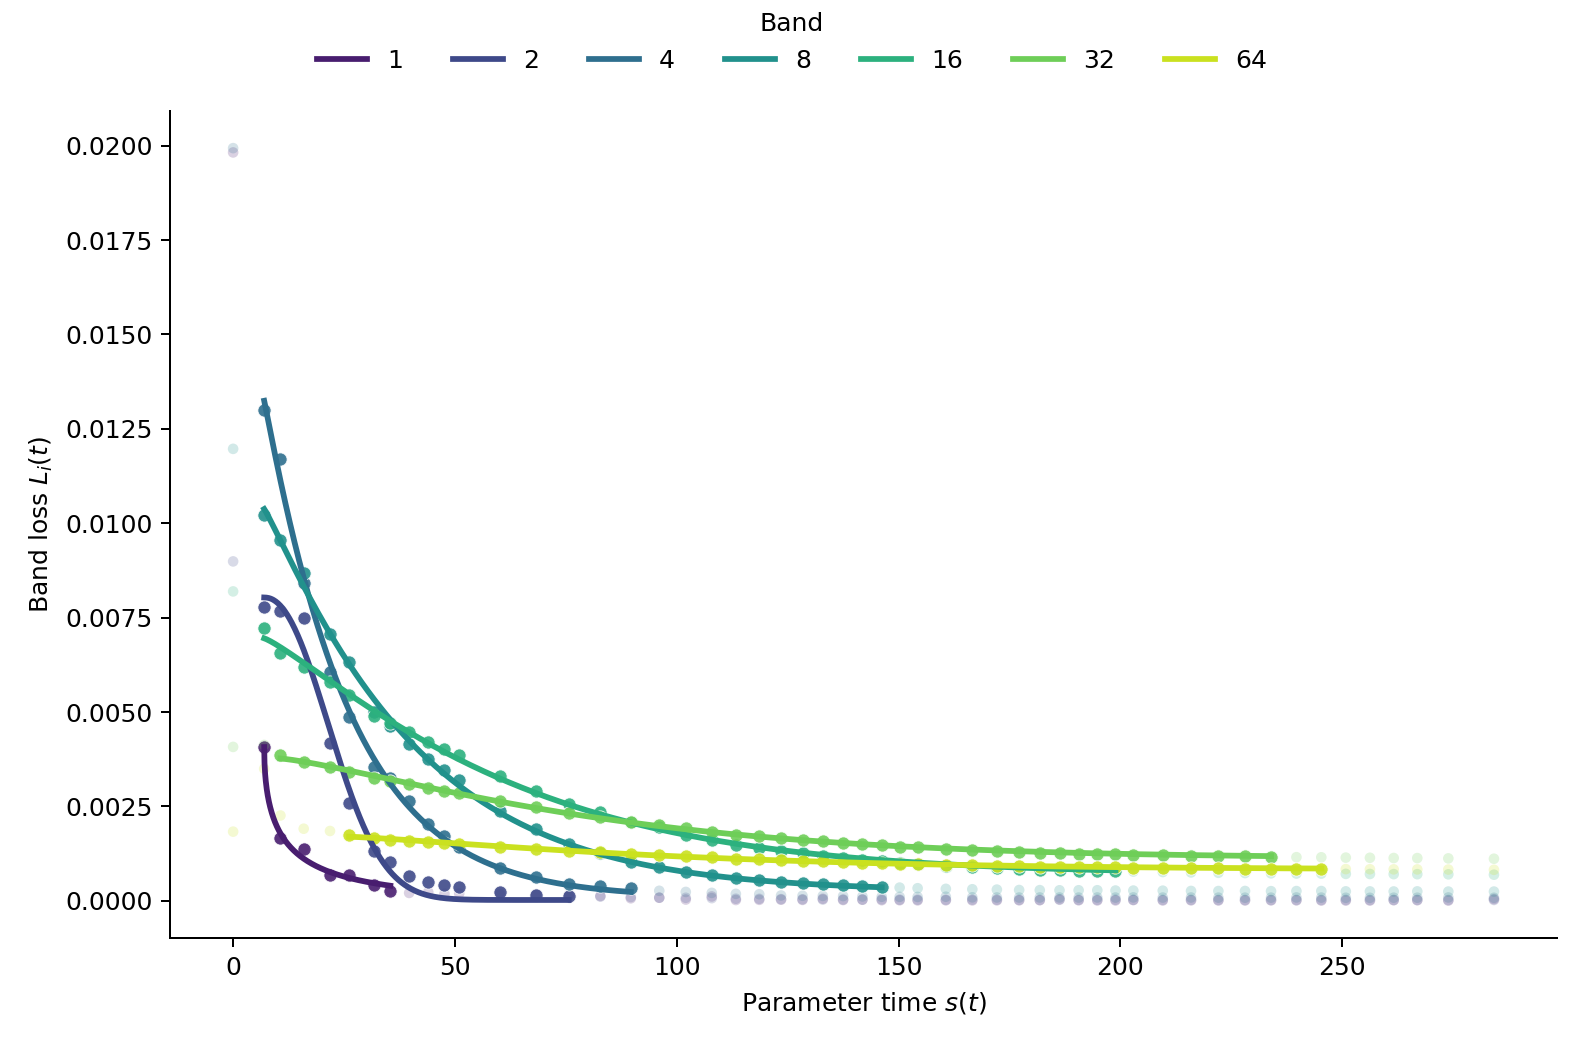
\includegraphics[width=0.6\linewidth]{figure3.png}
\caption{Weibull band fits for one representative run.
Dots are pale outside the active window.}
\label{fig:normalized-residuals}
\end{figure}

\subsection{Result 2: Band ordering}
\label{result-2-band-ordering}

We measure each band's onset $\tau_i = c_i(0.95)$, active width
$w_i = c_i(0.01) - c_i(0.95)$, initial residual $R_i(s_0)$, and floor
$L_i^\infty$ from its residual trajectory $R_i(s)$
(definitions in Section~\ref{experimental-setup}).
These crossing-based quantities are used for descriptive ordering; they
are not fitted parameters.

\begin{enumerate}
\item
  \textbf{Onset $\tau_i$}:
  finer bands activate later.
\item
  \textbf{Active width $w_i$}: finer bands decay over
  a wider $s$ window.
\item
  \textbf{Floor $L_i^\infty$}: finer bands plateau
  at higher asymptotic loss (i.e. more unresolved loss).
\item
  \textbf{Initial residual $R_i(s_0)$}: finer bands start with
  less loss available to resolve.
\end{enumerate}

Across the 12 runs, the run-level correlation summaries are:

\begin{center}
\small
\begin{tabular}{@{}lccc@{}}
\toprule
Descriptor & Median $\rho$ & IQR & Min--max \\
\midrule
Onset $\tau_i$ & 0.79 & [0.75, 0.79] & [0.75, 0.89] \\
Width $w_i$ & 0.96 & [0.96, 0.96] & [0.93, 1.00] \\
Floor $L_i^\infty$ & 0.96 & [0.96, 0.96] & [0.96, 0.96] \\
Initial residual $R_i(s_0)$ & $-0.89$ & [$-0.89$, $-0.88$] & [$-0.89$, $-0.82$] \\
\bottomrule
\end{tabular}
\end{center}

\subsection{Result 3: Full-loss Weibull}\label{result-3-global-fit-weibull}

Because the Haar bands are orthogonal and the loss is MSE, the
ordinary full-loss residual is the sum of the band residuals:
\[
R_{\mathrm{tot}}(s_k)=\sum_i R_i(s_k).
\]

We evaluate two quantities. 

First, we evaluate each per-band Weibull fit $\widehat R_i$ on the
full checkpoint grid and sum them to obtain the band-fit
reconstruction $\widehat R_{\Sigma}(s_k)=\sum_i \widehat R_i(s_k)$.
This matches $R_{\mathrm{tot}}$ with median $R^2=0.986$.

Second, we fit a single Weibull directly to $R_{\mathrm{tot}}$ over the
full checkpoint range, obtaining median $R^2=0.996$ and median
$\Delta\mathrm{BIC} = -28.83$ versus the exponential special case. As
noted in Prediction~3, the Weibull family is not closed under summation,
so this global fit is an empirical regularity rather than a consequence
of the bandwise fits.

The direct global fit splits by architecture: ViT is decisively
stretched ($\beta = 0.79$, $\Delta\mathrm{BIC} = -73.83$), while CNN is a
near-tie with exponential ($\beta \approx 0.95$,
$\Delta\mathrm{BIC} \approx +0.95$). At the per-band level both
architectures show $\beta > 1$ (bands 4--64), but CNN's sum of bands
composes to a shape closer to exponential while ViT's composes to a
stretched one.

\section{Discussion}\label{discussion}

We have proposed a methodology for studying training dynamics ---
decomposing loss by resolution band and reparameterizing time as
cumulative parameter distance --- and used it to test key search,
a phenomenological model of training
dynamics. The three predictions of key search are
supported by our 12-run CelebA training runs: per-band residuals follow Weibull
curves in parameter time, bands activate in a coarse-to-fine order with
predictable relationships between onset, width, floor, and initial residual,
and the full-loss residual is itself well described by a single Weibull.

The Weibull fits characterize the shape of per-band learning curves but
do not explain why training produces this shape. Key search provides one
interpretive frame; the empirical regularities may admit others. We do
not know which observations are consequences of the data, the
architecture, the optimizer, or their interaction: the CNN and ViT runs
share dataset and optimizer but differ in architecture, and while
per-band Weibull fits hold for both, the global fit shape differs
($\beta < 1$ only for ViT). We study a single dataset (CelebA
$64 \times 64$), a single task (autoencoding), and small models
(1.8--2.8M parameters) trained for 50 epochs; a thorough ablation has
not been performed.

The band-loss additivity that makes our decomposition exact relies on 
two properties: the Haar bands are
orthogonal and the loss is squared error. For cross-entropy loss ---
the standard in language modeling and classification --- no obvious analogous
Pythagorean decomposition exists, and it is unclear whether language
admits a natural orthogonal decomposition comparable to spatial
resolution bands for images. Extending this methodology to
cross-entropy settings therefore remains an open problem, not just
an engineering challenge. 

Several directions for future work follow naturally. First, systematic
ablations: varying the dataset (beyond CelebA, beyond faces), the
architecture (depth, width, convolutional vs.\ transformer vs.\ MLP),
and optimizer settings (learning rate, schedule, weight decay, SGD vs.\
Adam) to disentangle which aspects of the observed dynamics are
data-driven, architecture-driven, or optimizer-driven. Second, a more
careful comparison of parameter time to raw time, including how the
equation $s(t) \approx a + bt^\gamma$ varies across settings and
whether parameter-time Weibull fits can be related to existing raw-time
scaling laws \citep{kaplan2020scaling,hoffmann2022training}. Third, exploring whether ``keys''
in the key-search framework correspond to identifiable structures in the
network, connecting this work to mechanistic interpretability.

This paper contributes both a theory and a methodology. Key search
offers a framework in which training dynamics become predictable:
per-band residuals decay as Weibulls, bands activate coarse-before-fine,
and the full loss also has a Weibull shape. The methodology ---
decomposing loss into orthogonal resolution bands and reparameterizing
time as cumulative parameter distance --- provides a richer set of
observables than scalar loss alone, against which this and other
theories of learning can be formulated and tested.

\section*{Acknowledgments}

I would like to thank Luc Baracat and Marija Beljan for helpful discussions.

\bibliographystyle{plainnat}
\bibliography{references}

\appendix

\section{Experimental Details}\label{appendix:experimental-details}

\subsection{Data and Preprocessing}\label{app:data-preprocessing}

We use CelebA from HuggingFace (\texttt{nielsr/CelebA-faces}). Images
are center-cropped to $128\times 128$, then bilinearly resized to $64\times 64$
(align\_corners=False), and converted to tensors in $[0,1]$ via
\texttt{ToTensor()}. We apply no mean/std normalization and no data
augmentation. From the single HuggingFace train split, we use the first
182,599 images as our training set and the last 20,000 as the test set;
no separate validation set is held out.

\subsection{Architectures}\label{app:architectures}

\textbf{CNN autoencoder (1,829,379 parameters).} Encoder: four strided
convolutions ($3\to 32\to 64\to 128\to 256$ channels), each followed by ReLU;
flatten to a $256\times 4\times 4$ feature map; linear projection to a 128-dimensional
latent. Decoder: linear projection back to $256\times 4\times 4$, followed by four
transpose-convolutional layers ($256\to 128\to 64\to 32\to 3$), each followed
by ReLU except the final layer which uses Sigmoid.

\textbf{ViT autoencoder (2,779,651 parameters).} Encoder: patch size 4
(yielding $16\times 16$ = 256 patches), embedding dimension 192, 4 transformer
blocks, 6 attention heads, MLP ratio 4, GELU activation, learned
positional embeddings. Mean pooling followed by a linear projection to a
128-dimensional latent. Decoder is the same transpose-convolutional
stack as the CNN.

Both models are trained as plain autoencoders with pixel MSE
reconstruction loss.

\subsection{Training Configuration}\label{app:training-configuration}

Optimizer: plain Adam ($\beta_1=0.9$, $\beta_2=0.999$) with learning rate $3\times10^{-4}$ and no
learning-rate schedule, warmup, weight decay, gradient clipping, or
mixed precision. Training runs for 50 epochs at batch size 128, in
single-precision \texttt{float32} on CUDA.

\subsection{Runs and Seeds}\label{app:runs-seeds}

We train 12 runs in total: CNN and ViT architectures with seeds 45, 46,
47, 48, 49, 50 (12 runs = 6 CNN + 6 ViT). Each seed determines parameter
initialization, data ordering, and test-panel sampling.

\subsection{Checkpoint Schedule}\label{app:checkpoint-schedule}

Checkpoints are saved at 53 points per run, denser at the beginning to capture
early training dynamics. The exact schedule is:

\begin{itemize}
\tightlist
\item
  Epoch 0 (initialization).
\item
  Within epoch 1: epoch 1/32, 1/16, 1/8, 3/16, 1/4, 3/8, 1/2, 5/8, 3/4,
  7/8, 1.
\item
  Epochs 1.5 to 10: every 0.5 epoch.
\item
  Epochs 11 to 20: every epoch.
\item
  Epochs 22 to 42: every 2 epochs.
\item
  Epochs 45 and 50.
\end{itemize}

\subsection{Haar Decomposition}\label{app:haar-decomposition}

The Haar decomposition is computed offline from saved test-panel
reconstructions using a standard orthogonal 2D Haar pyramid. Band 1
corresponds to the final LL coefficient (coarsest), and bands 2, 4, 8,
16, 32, 64 correspond to increasingly fine detail subbands. Because the
decomposition is orthogonal, band losses sum exactly to total image MSE.

The Haar bands form an orthogonal decomposition of the image error. Let
the reconstruction error be

\[
e = x - f(x;\theta_t).
\]

Haar splits this error into separate resolution bands:

\[
e = e_1 + e_2 + e_4 + e_8 + \cdots,
\]

where each $e_i$ is the part of the error in band $i$.

The bands are orthogonal, meaning that different bands have zero inner
product:

\[
\langle e_i, e_{i'}\rangle = 0
\qquad \text{whenever } i \neq i'.
\]

In other words, the error in band $i$ does not overlap with the error
in band $i'$ under the pixel inner product. Pixel MSE is the average
squared error:

\[
\mathrm{MSE}(x,f(x;\theta_t))
=
\frac{1}{N}\sum_p e_p^2
=
\frac{1}{N}\langle e,e\rangle.
\]

Therefore, when we expand the squared error of the full image,

\[
\langle e,e\rangle
=
\left\langle \sum_i e_i,\sum_{i'} e_{i'} \right\rangle
=
\sum_i \langle e_i,e_i\rangle
+
\sum_{i\neq i'}\langle e_i,e_{i'}\rangle.
\]

The second term vanishes because the bands are orthogonal, so only the
within-band terms remain:

\[
\langle e,e\rangle
=
\sum_i \langle e_i,e_i\rangle.
\]

Dividing by $N$, the total image MSE becomes the sum of the band MSEs:

\[
\mathrm{MSE}(x,f(x;\theta_t))
=
\sum_i L_i(x,f(x;\theta_t)).
\]

This equality holds for each individual image and reconstruction pair,
not only on average over a dataset. It relies on two facts: the bands
must be orthogonal, and the loss must be squared error. If the bands are
not orthogonal, cross-terms like \(\langle e_1,e_2\rangle\) may be
nonzero, so the band losses no longer add exactly to the total loss. If
the loss is not squared error, such as L1 or cross-entropy, there is no
Pythagorean theorem that gives the same exact additive decomposition.

\subsection{Optimizer-Path Measurements}\label{app:optimizer-path-measurements}

Parameter time $s(t)$ is computed between saved checkpoints:

\[
s(t_k) = \sum_{m=1}^{k} \| \theta_m - \theta_{m-1} \|_2,
\]

where the sum is taken over all trainable parameters (no exclusions, no
per-layer normalization). Because $s$ is accumulated between saved
checkpoints rather than per optimizer step, it approximates the true
optimizer path by chord lengths between checkpoints. This slightly
underestimates the true arc length but preserves the relative ordering
of checkpoints, which is what the analyses in this paper require.

Empirically, parameter time is well fit as a power of raw time,
$s(t) \approx a + b \cdot t^\gamma$. Using a three-parameter nonlinear
fit over the full 50-epoch window, the median exponent is
$\gamma = 0.368$, with SD $= 0.008$ across runs and median
$R^2 = 0.999$. The exponent is different across architectures and window sizes.
So $\gamma$ is best read as a window-specific parameter rather
than a universal constant.

\begin{center}
\small
\begin{tabular}{@{}lcccc@{}}
\toprule
Window & Architecture & Runs & Median $\gamma$ & Median $R^2$ \\
\midrule
0--10  & CNN & 6 & 0.354 & 0.999 \\
0--25  & CNN & 6 & 0.371 & 1.000 \\
0--50  & CNN & 6 & 0.370 & 1.000 \\
0--10  & ViT & 6 & 0.472 & 0.999 \\
0--25  & ViT & 6 & 0.412 & 0.999 \\
0--50  & ViT & 6 & 0.365 & 0.999 \\
\bottomrule
\end{tabular}
\end{center}

\subsection{Evaluation Panel}\label{app:evaluation-panel}

Each run has a fixed evaluation panel of 256 images, sampled without
replacement from the 20,000 images test split using RNG seed (seed + 3).
The panel is fixed across all checkpoints within a run but not shared
across runs. Panel reconstructions are stored as float16 NumPy archives.

\subsection{Floors}\label{app:floors}

The band floor $L_i^\infty$ is the mean band loss over the last five
saved checkpoints. The full-loss floor is the sum of the band floors,
$L_{\mathrm{tot}}^\infty=\sum_i L_i^\infty$, so that the additivity
$R_{\mathrm{tot}}(s_k)=\sum_i R_i(s_k)$ holds exactly. For comparison,
the late-checkpoint average differs from the final-checkpoint floor by
at most 0.51\% of each band's full dynamic range across all run--band
pairs, so the two conventions are effectively interchangeable for this
dataset.

\subsection{Threshold Crossings}\label{app:crossings}
The $\alpha$-crossing $c_i(\alpha)$ (defined in
Section~\ref{threshold-crossings}) is estimated by linear interpolation:
if $q_i(s_{k-1})>\alpha$ and $q_i(s_k)\leq\alpha$, then
\[
c_i(\alpha)
=s_{k-1}
+\frac{q_i(s_{k-1})-\alpha}{q_i(s_{k-1})-q_i(s_k)}
\left(s_k-s_{k-1}\right).
\]

The interpolation is used only to estimate crossing times. For per-band
fits, the window starts at the first saved checkpoint after \(c_i(0.95)\) and ends at the
last saved checkpoint before \(c_i(0.01)\). No interpolated residual or
loss values enter the least-squares objective. Direct global fits to
\(R_{\mathrm{tot}}\) use the full saved-checkpoint range with no
threshold trimming.

\subsection{BIC Calculation}\label{app:bic-calculation}

BIC is computed from the same checkpoint values and the same
linear-scale least-squares objective used for fitting. For fitted values
\(\widehat R(s_k)\) on \(n\) saved checkpoints, let
\[
\mathrm{SSE}=\sum_{k=1}^{n}\left(R(s_k)-\widehat R(s_k)\right)^2.
\]

The full BIC formula is
\[
\mathrm{BIC}
=
n\log\!\left(\frac{\mathrm{SSE}}{n}\right)
+ p\log n
+ n\log(2\pi) + n.
\]

The last two terms cancel in

\[
\Delta\mathrm{BIC}
=
\mathrm{BIC}_{\mathrm{Weibull}}
-
\mathrm{BIC}_{\mathrm{exp}},
\]

so we compute BIC in a reduced form

\[
\mathrm{BIC}
=
n\log\!\left(\frac{\mathrm{SSE}}{n}\right)
+ p\log n.
\]
The Weibull fit has $p=3$ parameters $(A,\omega,\beta)$; the exponential
baseline fixes $\beta=1$ and has $p=2$ parameters $(A,\omega)$.

\subsection{Software and AI Assistance}\label{app:software}

PyTorch 2.7.1, HuggingFace Datasets, NumPy, Pandas, SciPy, PIL. Fitting
uses \texttt{scipy.optimize.}\allowbreak\texttt{least\_squares}.
Public code and derived clean artifacts are available at
\url{https://github.com/jurij-jukic/key_search_paper_code}.
Heavyweight checkpoints and panel dumps are referenced by manifests and
can be materialized separately.

OpenAI's GPT 5.4 and 5.5 were used for orchestrating training runs,
and writing the analysis code. Writing this paper was assisted by
Anthropic's Claude 4.6, 4.7, and OpenAI's GPT 5.4 and 5.5.

\subsection{Hardware and Runtime}\label{app:hardware-runtime}

Training runs on NVIDIA GPUs (RTX 3090-class; exact model varies by
launch manifest). Median per-run wall-clock time: 24 minutes for CNN
runs, 89 minutes for ViT runs. Total compute for the 12-run pilot:
approximately 12 GPU-hours.

\section{Weibull Fit Details}\label{appendix:weibull-fit-details}

\subsection{Fit Form and Procedure}\label{app:fit-procedure}

We fit the Weibull form

\begin{equation}\label{eq:fit-form}
R_i(s) = A \cdot \exp\!\left(-((s - s_{\text{start}})/\omega)^\beta\right),
\end{equation}

where $A$ is the fitted active-window amplitude, not necessarily the
initial residual $R_i(s_0)$. We use \texttt{scipy.optimize.least\_squares}
with parameter bounds $A > 0$, $\omega > 0$, $\beta \in [0.05, 8]$. The optimizer
is multistarted from several initial parameter guesses to reduce
sensitivity to local minima.

For each band, the active window is selected using the crossings
defined in Appendix~\ref{app:crossings}. Within this window,
$s$ is rebased so that the first fitted checkpoint has \(s=0\).

\subsection{Per-Band Weibull vs. Exponential}\label{app:per-band-weibull-vs-exponential}

For each of 84 run-band fits (12 runs $\times$ 7 bands), we compare Weibull
against pure exponential ($\beta = 1$ in the same window) via BIC.

\textbf{Overall:} median $R^2 = 0.997$, median $\Delta\mathrm{BIC} = -19.65$, Weibull
preferred in 72/84 fits.

\textbf{Per-band medians (across 12 runs):}

\begin{center}
\small
\begin{tabular}{@{}lcccccc@{}}
\toprule
Band & $R^2$ & $\beta$ & $\Delta\mathrm{BIC}$ & Wins & $\Delta\mathrm{BIC}$ ($n/10$) & Wins ($n/10$) \\
\midrule
1  & 0.982 & 0.90 & $+1.14$  & 4/12  & $-0.52$ & 12/12 \\
2  & 0.992 & 3.13 & $-19.05$ & 11/12 & $-1.97$ & 12/12 \\
4  & 0.995 & 1.31 & $-3.58$  & 10/12 & $-0.49$ & 8/12 \\
8  & 0.996 & 1.29 & $-9.27$  & 12/12 & $-0.80$ & 11/12 \\
16 & 0.998 & 1.28 & $-50.63$ & 12/12 & $-4.28$ & 12/12 \\
32 & 0.999 & 1.26 & $-70.92$ & 12/12 & $-6.03$ & 12/12 \\
64 & 0.999 & 1.16 & $-35.44$ & 11/12 & $-2.49$ & 11/12 \\
\bottomrule
\end{tabular}
\end{center}

Weibull is decisively preferred over exponential from band 8 upward.
Bands 4--64 show $\beta$ consistently above 1 (initial shoulder and then
decay), with $\beta \in [1.16, 1.31]$.

Two coarse bands are less clean: band 1's shape is not distinguishably
non-exponential, and band 2 has an inflated $\beta = 3.1$. Both issues likely
stem from sparse early checkpoints combined with optimizer instability
in the first epoch, when these bands are decaying fastest.

\textbf{Robustness to effective sample size.} Adjacent checkpoints are
temporally correlated, so nominal $N$ overestimates effective sample size.
Under the conservative adjustment $n_{\mathrm{eff}} = n/10$, bands 16 and 32 remain
decisive ($|\Delta\mathrm{BIC}| > 4$); other bands become
marginal but Weibull still wins the majority at every band (78/84
overall, median $\Delta\mathrm{BIC} = -1.73$).

\subsection{Robustness to Fit-Window Choice}\label{app:fit-window-robustness}

We test whether the conclusions for each band depend on the particular
active-window thresholds by repeating the analysis with two narrower
windows, 0.90/0.10 and 0.80/0.20, in addition to the primary 0.95/0.01
window. 

\subsubsection{Per-Band Weibull Fits}\label{app:robustness-per-band-fits}

Medians across runs under three threshold windows (left edge / right
edge). In some cases the medians are applied to less than 12 runs because
some runs under narrower windows don't have enough checkpoints to make
the data reliable. When there is less than five checkpoints inside the 
window, the data is omitted.

\begin{center}
\footnotesize
\resizebox{\textwidth}{!}{%
\begin{tabular}{@{}lccccccccc@{}}
\toprule
Band & $R^2$ (.95/.01) & $\beta$ (.95/.01) & $\Delta\mathrm{BIC}$ (.95/.01) &
$R^2$ (.90/.10) & $\beta$ (.90/.10) & $\Delta\mathrm{BIC}$ (.90/.10) &
$R^2$ (.80/.20) & $\beta$ (.80/.20) & $\Delta\mathrm{BIC}$ (.80/.20) \\
\midrule
1  & 0.982 & 0.90 & $+1.14$  & ---   & ---  & ---      & ---   & ---  & --- \\
2  & 0.992 & 3.13 & $-19.05$ & 0.979 & 2.62 & $-11.88$ & ---   & ---  & --- \\
4  & 0.995 & 1.31 & $-3.58$  & 0.994 & 1.36 & $-3.60$  & 0.993 & 1.60 & $-5.47$ \\
8  & 0.995 & 1.29 & $-9.27$  & 0.993 & 1.32 & $-5.05$  & 0.994 & 1.03 & $+1.47$ \\
16 & 0.998 & 1.28 & $-50.63$ & 0.997 & 1.21 & $-14.09$ & 0.997 & 1.10 & $-8.63$ \\
32 & 0.999 & 1.26 & $-70.92$ & 0.999 & 1.29 & $-45.73$ & 0.999 & 1.22 & $-19.37$ \\
64 & 0.999 & 1.16 & $-35.44$ & 0.999 & 1.17 & $-36.09$ & 1.000 & 1.19 & $-38.79$ \\
\bottomrule
\end{tabular}%
}
\end{center}

Fit quality ($R^2$) is stable across thresholds. $\Delta\mathrm{BIC}$ magnitudes change but
Weibull preference remains strong for bands 16--64; band 8 becomes
slightly exponential-favored under the narrowest 0.80/0.20 window.

\subsubsection{Band Ordering}\label{app:robustness-band-ordering}

Within-run Spearman correlations across 12 runs.
\begin{center}
\small
\begin{tabular}{@{}llccc@{}}
\toprule
Metric & Window & Median $\rho$ & IQR & Min--max \\
\midrule
Onset $\tau_i$ & 0.95/0.01 & 0.786 & [0.750, 0.786] & [0.750, 0.893] \\
Onset $\tau_i$ & 0.90/0.10 & 0.786 & [0.750, 0.786] & [0.750, 0.893] \\
Onset $\tau_i$ & 0.80/0.20 & 0.804 & [0.750, 0.929] & [0.750, 0.964] \\
Width $w_i$ & 0.95/0.01 & 0.964 & [0.964, 0.964] & [0.929, 1.000] \\
Width $w_i$ & 0.90/0.10 & 1.000 & [0.964, 1.000] & [0.964, 1.000] \\
Width $w_i$ & 0.80/0.20 & 1.000 & [1.000, 1.000] & [0.964, 1.000] \\
Floor $L_i^\infty$ & 0.95/0.01 & 0.964 & [0.964, 0.964] & [0.964, 0.964] \\
Floor $L_i^\infty$ & 0.90/0.10 & 0.964 & [0.964, 0.964] & [0.964, 0.964] \\
Floor $L_i^\infty$ & 0.80/0.20 & 0.964 & [0.964, 0.964] & [0.964, 0.964] \\
Initial residual $R_i(s_0)$ & 0.95/0.01 & $-0.893$ & [$-0.893$, $-0.875$] & [$-0.893$, $-0.821$] \\
Initial residual $R_i(s_0)$ & 0.90/0.10 & $-0.893$ & [$-0.893$, $-0.875$] & [$-0.893$, $-0.821$] \\
Initial residual $R_i(s_0)$ & 0.80/0.20 & $-0.893$ & [$-0.893$, $-0.875$] & [$-0.893$, $-0.821$] \\
\bottomrule
\end{tabular}
\end{center}

Onset, width, floor, and initial-residual correlations are essentially
invariant to threshold choice.

\section{Notation}\label{appendix:notation}

{\small
\begin{longtable}{@{}>{\raggedright\arraybackslash}p{0.23\linewidth}>{\raggedright\arraybackslash}p{0.72\linewidth}@{}}
\toprule\noalign{}
Symbol & Meaning \\
\midrule\noalign{}
\endhead
\bottomrule\noalign{}
\endlastfoot
\multicolumn{2}{l}{\textbf{Data and model}} \\
$x$ & Input image \\
$f(x;\theta_t)$ & Model reconstruction of $x$ at training time $t$ \\
$\theta_t$ & Model parameters at training time $t$ \\
$e$ & Reconstruction error, $e = x - f(x;\theta_t)$ \\
$N$ & Number of pixels per image \\
\\
\multicolumn{2}{l}{\textbf{Time}} \\
$t$ & Raw training time (step count) \\
$s(t)$ & Parameter time: cumulative Euclidean distance by raw step $t$ \\
$k$ & Checkpoint index \\
$s_k$ & Parameter time at saved checkpoint $k$ \\
$s_0$ & Parameter time at the initial checkpoint \\
\\
\multicolumn{2}{l}{\textbf{Resolution bands}} \\
$i$ & Band index; bands correspond to spatial scales $r\in\{1,2,4,8,16,32,64\}$ \\
$e_i$ & Reconstruction error in band $i$ \\
\\
\multicolumn{2}{l}{\textbf{Loss and residuals}} \\
$L_i(s)$ & Band loss: MSE restricted to band $i$ at time $s$ \\
$L_i^\infty$ & Band floor: mean loss over the last five saved checkpoints in band $i$ \\
$L_{\mathrm{tot}}(s)$ & Total loss at time $s$: $\sum_i L_i(s)$ \\
$L_{\mathrm{tot}}^\infty$ & Total floor: $\sum_i L_i^\infty$ \\
$R_i(s)$ & Band residual: $L_i(s) - L_i^\infty$ \\
$R_i(s_0)$ & Initial residual in band $i$, used for band ordering \\
$R_{\mathrm{tot}}(s)$ & Total residual: $\sum_i R_i(s) = L_{\mathrm{tot}}(s) - L_{\mathrm{tot}}^\infty$ \\
\\
\multicolumn{2}{l}{\textbf{Weibull fits and comparisons}} \\
$A$ & Fitted active-window amplitude in Eq.~\eqref{eq:fit-form} \\
$\omega$ & Weibull scale parameter \\
$\beta$ & Weibull shape parameter \\
$BIC$ & Bayesian Information Criterion \\
$\Delta\mathrm{BIC}$ & $\mathrm{BIC}_{\mathrm{Weibull}}-\mathrm{BIC}_{\mathrm{exp}}$; negative favors Weibull \\
$\widehat R_i$ & Weibull fit for band $i$ \\
$\widehat R_\Sigma$ & Band fit reconstruction: $\sum_i\widehat R_i$ \\
\\
\multicolumn{2}{l}{\textbf{Threshold crossings}} \\
$q_i(s_k)$ & Normalized residual: $R_i(s_k)/R_i(s_0)$ \\
$\alpha$ & Threshold level \\
$c_i(\alpha)$ & $\alpha$-crossing: interpolated parameter time at which $q_i$ first falls below $\alpha$ \\
$\tau_i$ & Onset: $c_i(0.95)$ \\
$w_i$ & Active width: $c_i(0.01) - c_i(0.95)$ \\
\\
\multicolumn{2}{l}{\textbf{Weibull tail (theory)}} \\
$T_i(x)$ & Tail function for band $i$ \\
$A_i^{\mathrm{tail}}$ & Theoretical tail amplitude in Eq.~\eqref{eq:weibull-tail} \\
$x_i(t)$ & Frontier position (latent) for band $i$ \\
$\ell$ & Key length in the key-search model \\
\\
\end{longtable}
}

\end{document}
